\chapter{Introduction}

\framedt{Preface}{
This is the report of the exam project of the \textit{Peer-to-Peer and Blockchain} UniPi course. The assignment consisted in developing a solidity-based version of the famous Mastermind game.\\
\ul{The project may be found at} \href{https://github.com/frenzis01/mastermind}{github.com/frenzis01/mastermind} \ul{along with a brief \textit{demo}}.
The developed application consists of a Solidity backend exploiting the \textit{Hardhat} framework, and a \textit{Vite} react-based frontend.
The project was jointly developed by \textbf{Emiliano Sescu} and \textbf{Francesco Lorenzoni}; aside from the contribution and commit history itself, we discussed together almost all design choices and shared with each other the implementations aspects learned throughout the development.\\
For instructions on how to deploy the contract and interact with it using the frontend, please refer to the \texttt{README} file located in the project's GitHub repository.
}
\nl

Mastermind is a two-player code-breaking game where one player (the code \textmauve{maker}) creates a secret code using colored pegs,
and the other player (the code \textgreen{breaker}) tries to guess the code within a fixed number of guesses. 
After each guess, the code \textmauve{maker} provides feedback with key pegs: black for correct color and position, white for correct color but wrong position.
The code \textgreen{breaker} wins a turn by guessing the code within the allowed number of guesses; otherwise, the code \textmauve{maker} wins.

\section{Overview}

Players can join the platform by connecting their Metamask Wallet. Once connected, they will be able to use wallet's profiles to log in using a specific address.
Note that due to the way wallets are integrated in Metamask, \ul{each operation on the blockchain requiring a fee results in a transaction to be confirmed in a wallet pop-up}.

From the home page, players can either \textbf{create} a game, \textbf{join} new games
% (TODO: specificare la cosa dello stake. Fatto sotto)
or \textbf{resume} previously started ones, as shown in Figure \ref{fig:home}. Players have the flexibility to leave and rejoin any ongoing game at any time.
Highlighted games represent challenges directed to a specific address, which are only visible to the challenged address.
\ul{There is no handshake protocol between creator and joiner to establish the stake for a game, every player may create a game proposing a stake, and every joiner is free to choose which stake fits best its needs.}
% NOTA il creator però intanto paga lo stake per creare il gioco

\begin{figure}[htbp]
   \centering
   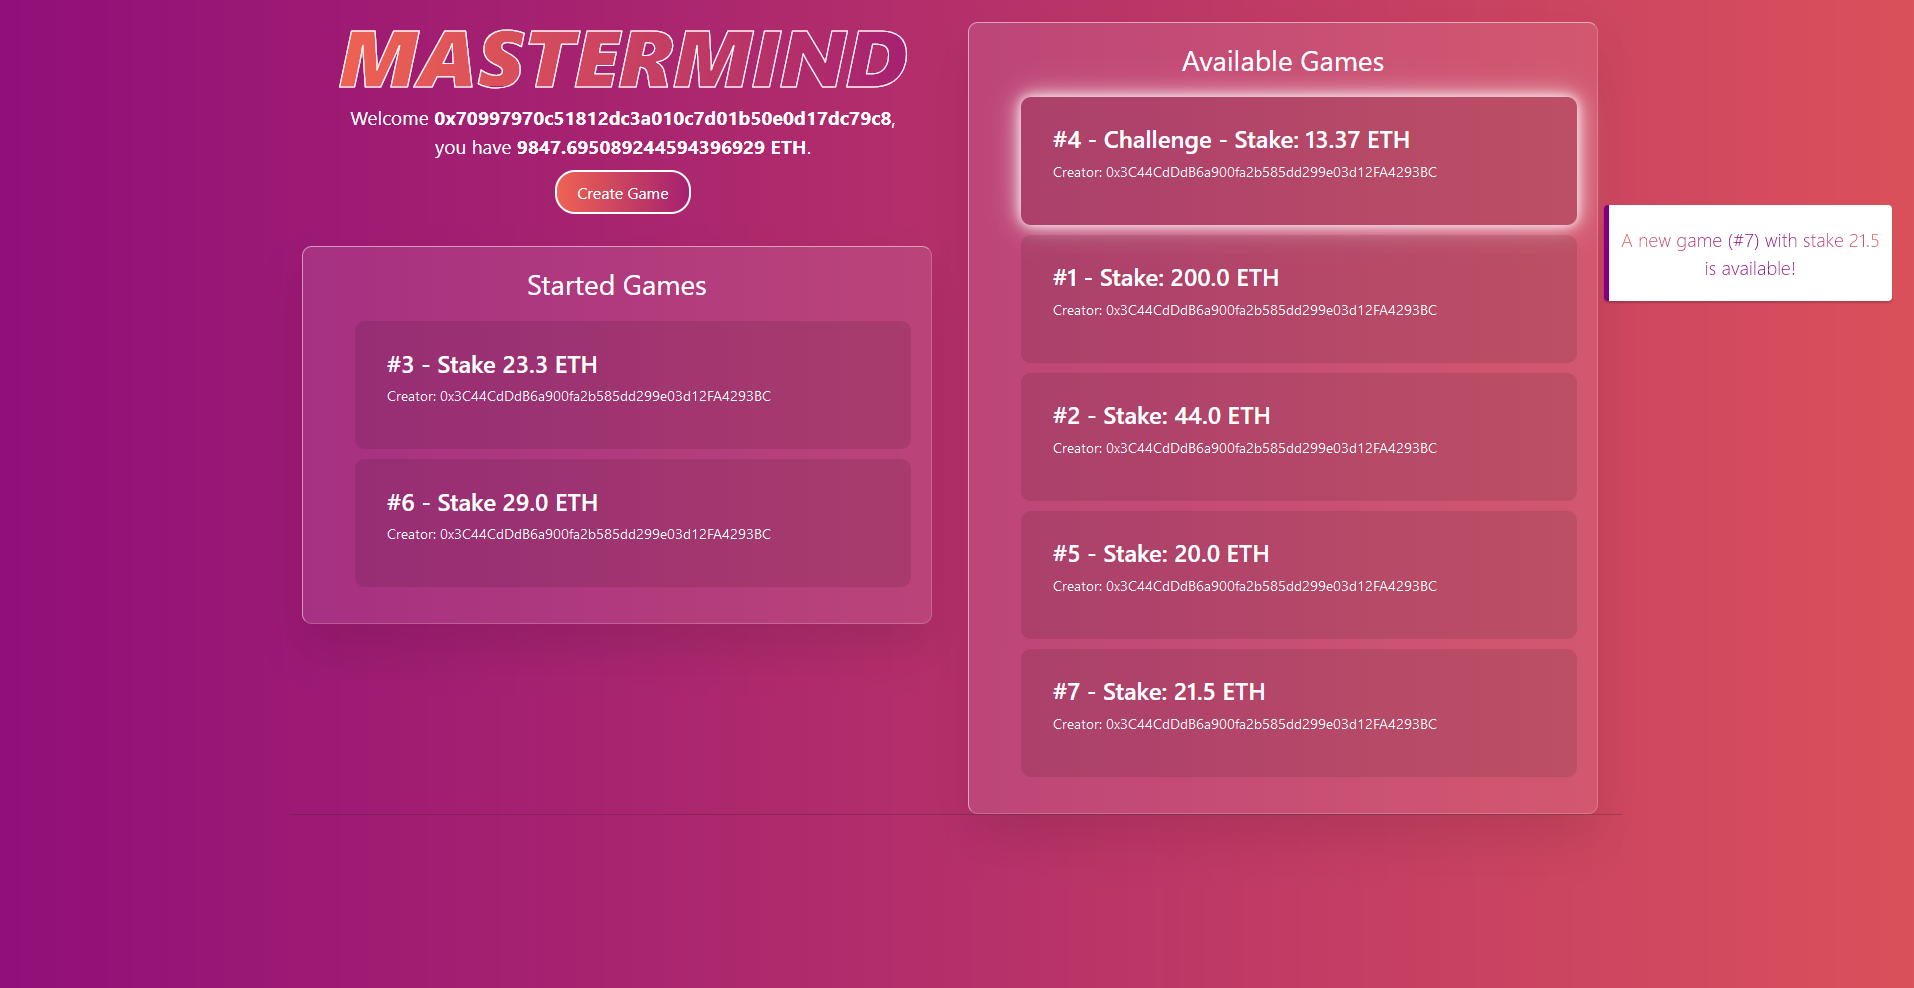
\includegraphics{images/home.PNG}
   \caption{Home page}
   \label{fig:home}
\end{figure}

\newpage
% edited
When a player creates a game, a role of either ``\textmauve{maker}" or ``\textgreen{breaker}" is randomly assigned; the two boards displayed corresponding to each role are similar, but expose to the user different interactions according to the role assigned. The game creator will be notified of the join when an opponent joins the game; similar notifications are sent for each in-game event. 
The \textgreen{breaker}, regardless of whether they are creator or joiner, always starts the turn, while the \textmauve{maker} waits for the \texttt{TurnStarted} event. 
Upon receiving the event, the \textmauve{maker} selects a secret code, prepends a \textit{salt}, and publishes the hash onto the blockchain using the modal shown in Figure \ref{fig:maker_secret_code}.
The \textgreen{breaker} will receive the hash publication \texttt{HashPublished}, and the turn will start.

\begin{figure}[htbp]
   \centering
   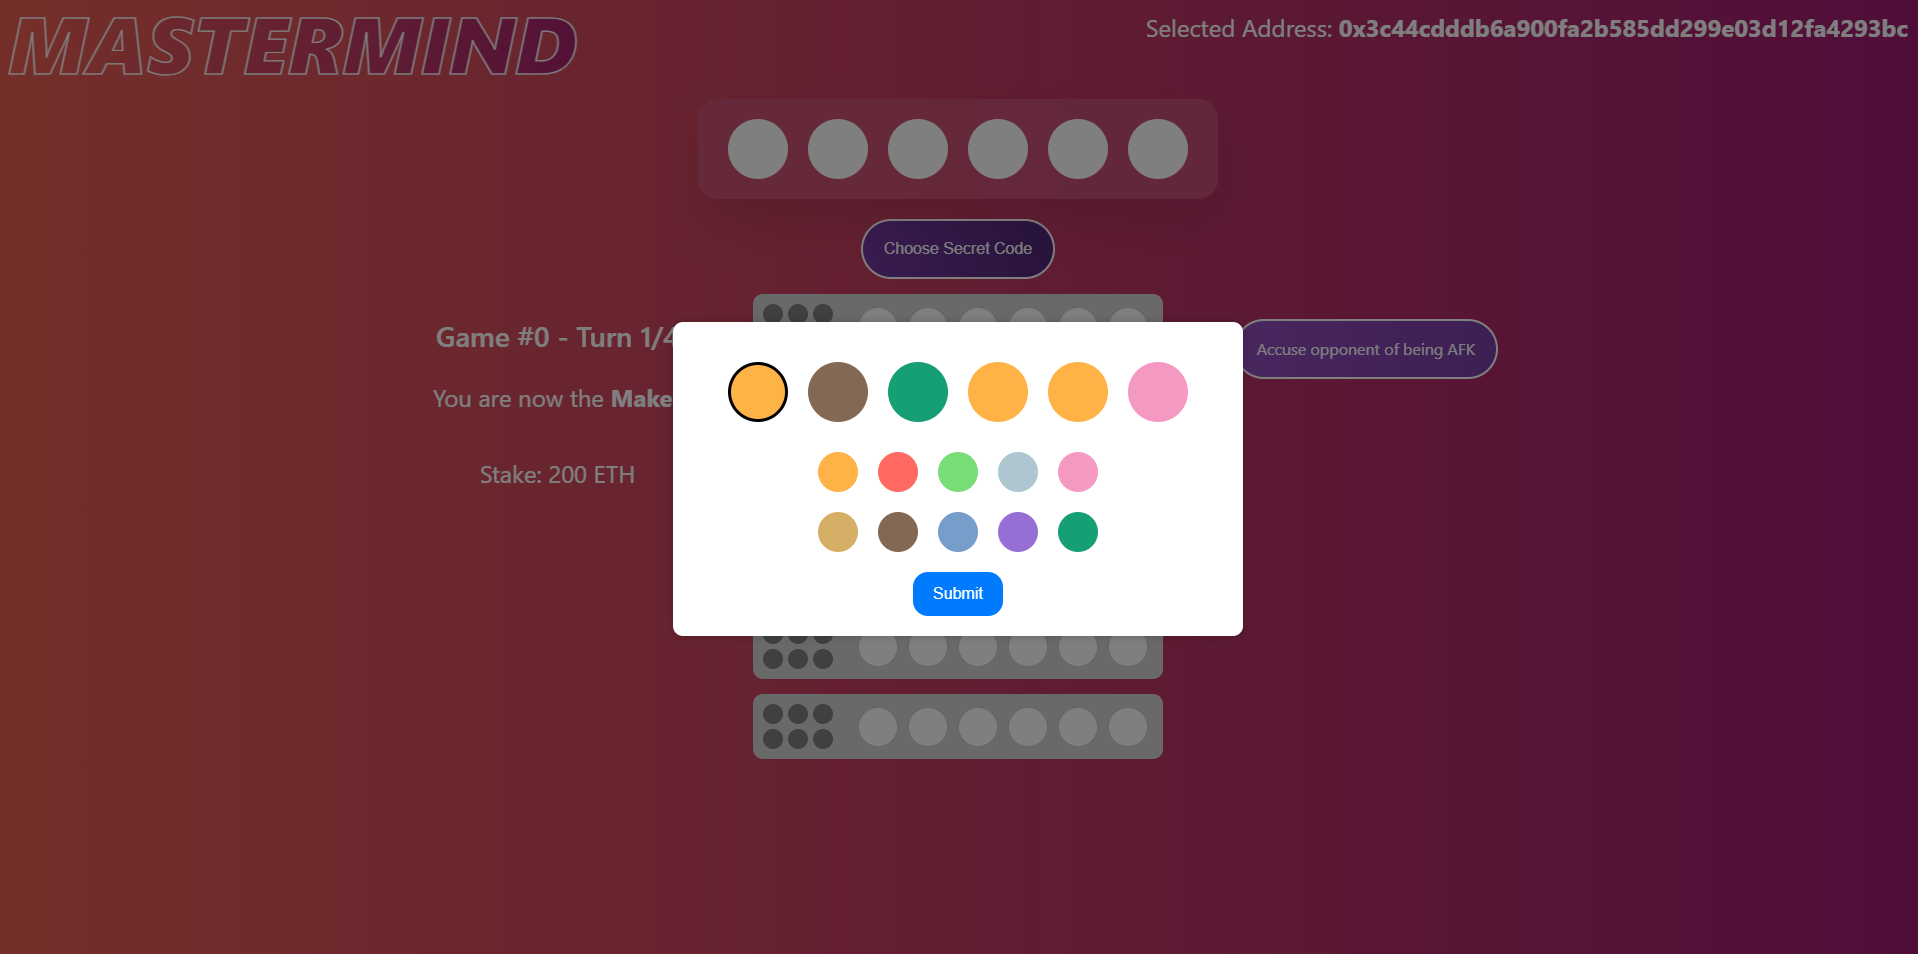
\includegraphics{images/board maker.PNG}
   \caption{\textmauve{maker} selects secret code}
   \label{fig:maker_secret_code}
\end{figure}

% edited
The \textgreen{breaker} uses a similar modal to make guesses, and, upon the receival of a \texttt{Guess} the \textmauve{maker} provides the corresponding feedback (a tuple $\langle \texttt{CC/NC} \rangle $).
The rows in the board get colored according to received guesses and feedbacks which are all stored in the blockchain, allowing for game interruption and later resume.

At any point, a player can accuse the opponent of being \textbf{AFK} (\textit{Away From Keyboard}) using the \textit{``Accuse opponent of being AFK"} button. 
The accused player then has a limited number of blocks to perform a game action; 
the accuser can at any time check whether the ``time"  has elapsed, i.e. the opponent is not playing and went AFK.
In this case the accuser wins the entire game stake, otherwise the game normally proceeds.

\newpage
Once the \textgreen{breaker} either guesses the code or exhausts their attempts, the \textbf{turn} concludes. The \textmauve{maker} must then publish the secret code in clear text along with the salt. 
The blockchain verifies that the $hash(salt|code)$ matches the initially published hash. If there is a discrepancy, the current \textgreen{breaker} claims the entire game stake. 
The \textgreen{breaker} then validates the feedbacks received (Figure \ref{fig:breaker_secret_code}); if some feedbacks are deemed invalid, they may dispute them and claim the stake if the dispute is correct; 
Note that if the \textgreen{breaker} disputes $fb_1,fb_3,...fb_k$ and at least one of them was correct, the \textmauve{maker} wins the game and obtains the stake.

\begin{figure}[htbp]
   \centering
   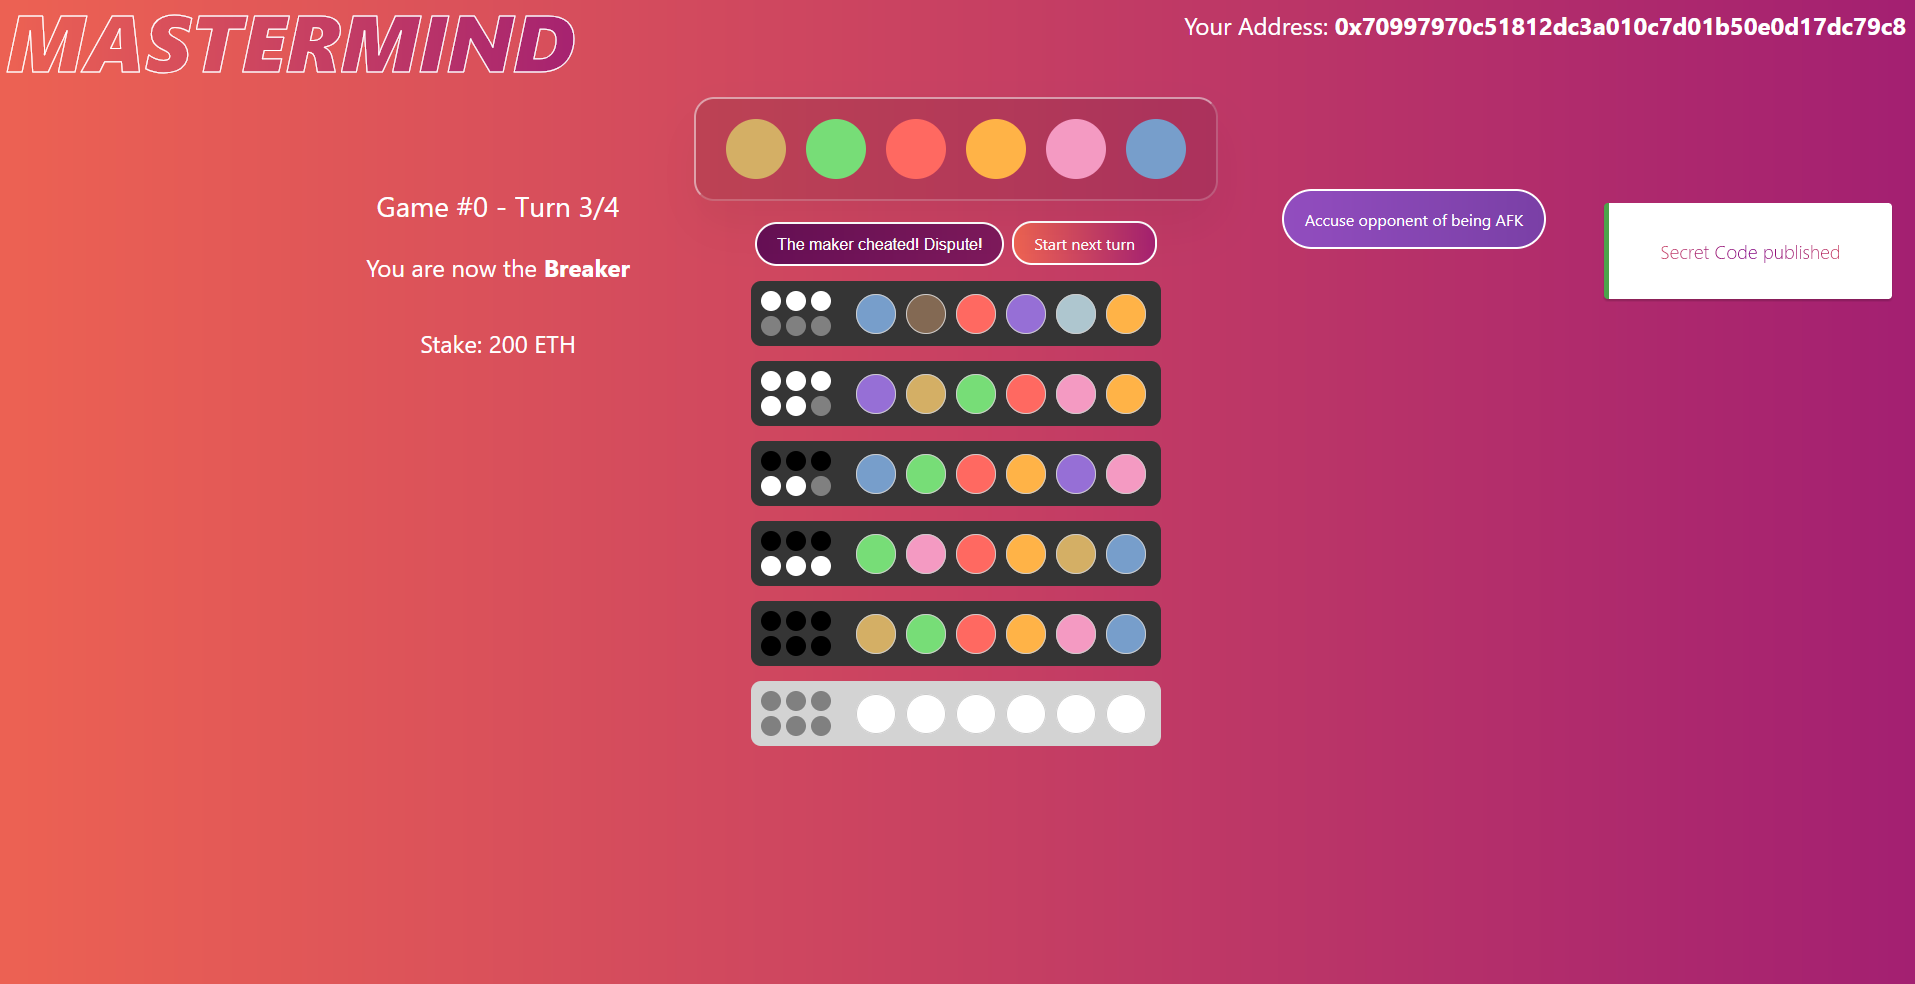
\includegraphics{images/board breaker.PNG}
   \caption{\textgreen{breaker} receives secret code}
   \label{fig:breaker_secret_code}
\end{figure}

At the end of each turn, points are awarded to the \textmauve{maker} based on the number of guesses the \textgreen{breaker} needed to crack the code. 
Additional points are given if the \textgreen{breaker} uses all their attempts without guessing the code. 
After all turns have been played, the player with more points is declared the winner and receives the entire stake, as shown in Figure \ref{fig:win_interface}.
\note{In case of a tie, the creator wins.}

\begin{figure}[htbp]
   \centering
   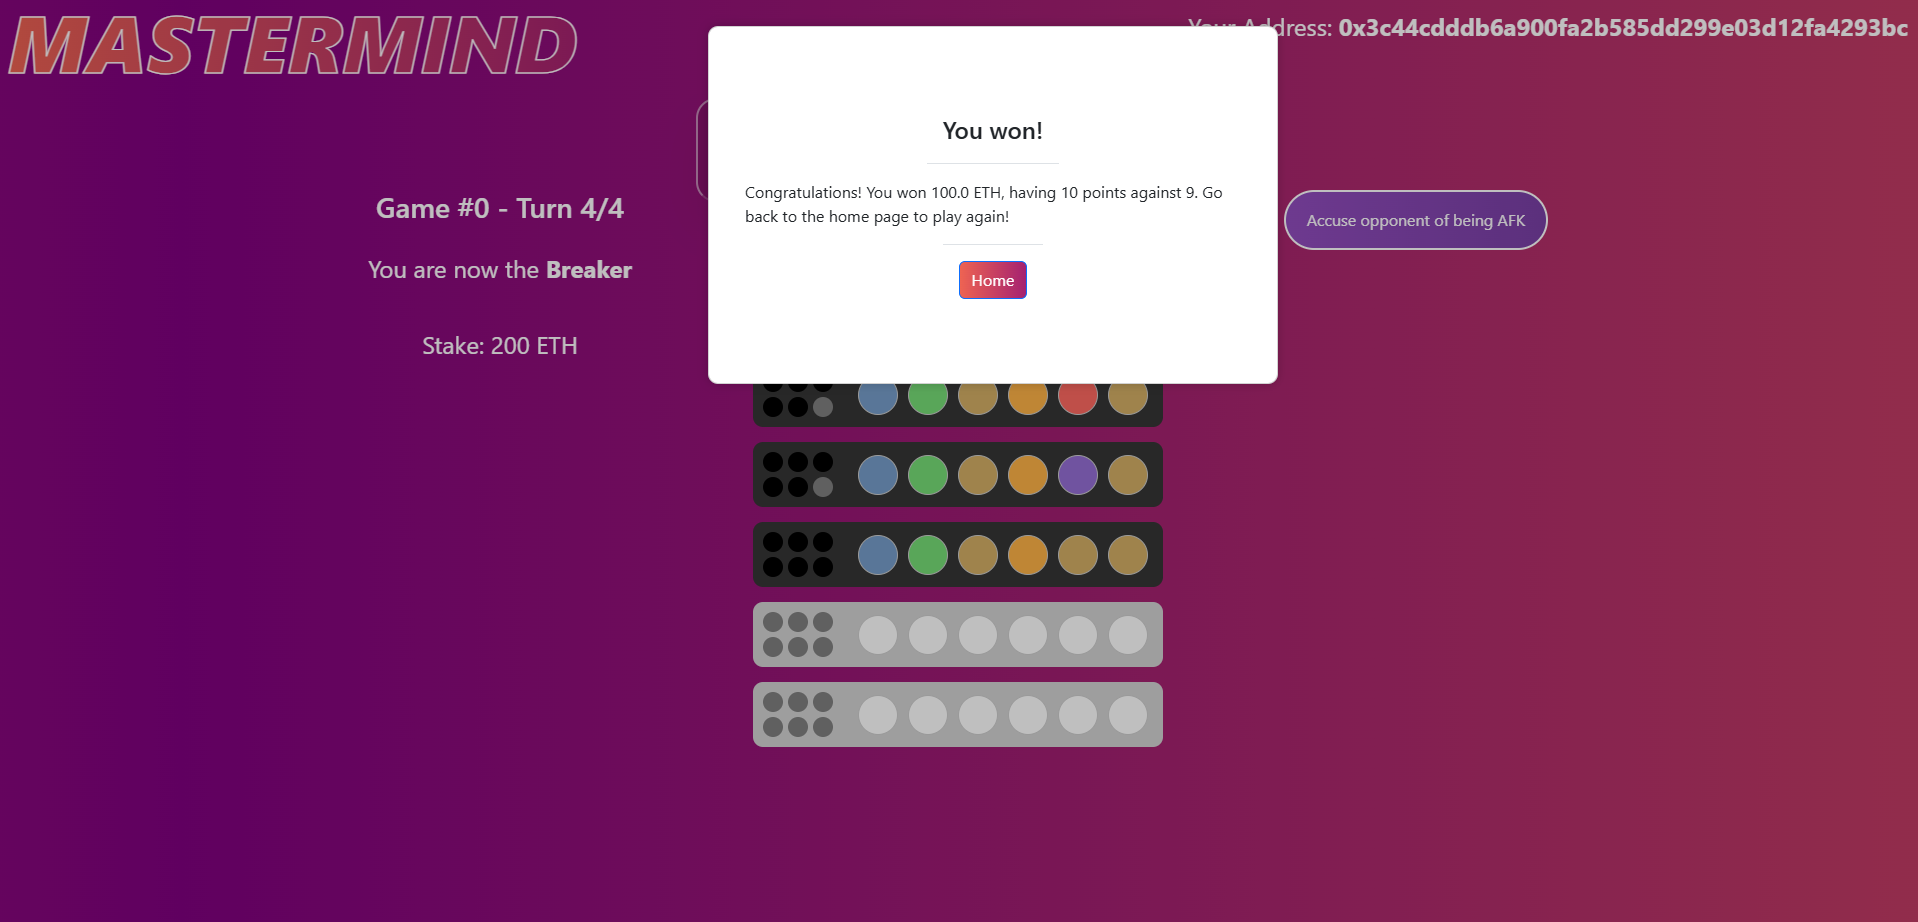
\includegraphics{images/win.PNG}
   \caption{Win modal}
   \label{fig:win_interface}
\end{figure}

